\documentclass[11pt,a4paper]{article}
\usepackage[utf8]{inputenc}
\usepackage[T1]{fontenc}
\usepackage[brazil]{babel}
\usepackage{lmodern}
\usepackage[margin=2cm]{geometry}
\usepackage{amsmath,amssymb}
\usepackage{booktabs}
\usepackage{graphicx}
\usepackage{hyperref}
\usepackage{xcolor}
\usepackage{titlesec}
\usepackage{tabularx}
\usepackage{enumitem}
\usepackage{float}
\usepackage{array}
\renewcommand{\tabularxcolumn}[1]{>{\raggedright\arraybackslash}p{#1}}

\hypersetup{
    colorlinks=true,
    linkcolor=blue!70!black,
    citecolor=blue!70!black,
    urlcolor=blue!70!black
}

\titleformat{\section}{\large\bfseries}{\thesection.}{0.5em}{}
\titleformat{\subsection}{\normalsize\bfseries}{\thesubsection.}{0.5em}{}
\titlespacing*{\section}{0pt}{1.2ex plus 0.5ex minus .2ex}{0.6ex}
\titlespacing*{\subsection}{0pt}{1.0ex plus 0.4ex minus .2ex}{0.4ex}

\setlength{\parskip}{0.45em}
\setlength{\parindent}{0pt}
\setlist{itemsep=0.15em,topsep=0.3em}

\begin{document}

\begin{center}
    {\LARGE \textbf{Relatório de Status do TCC}} \\[0.35em]
    {\large Avaliação das Explicações SHAP em Redes Neurais Profundas para Classificação de Arritmias Cardíacas em ECG} \\[0.3em]
    \textbf{Aluno:} Arthur Santos de Oliveira (RA: 156297) \\[0.2em]
    \textbf{Orientador:} Prof.\ Dr.\ Luis Augusto Martins Pereira \\[0.2em]
    \textbf{Data:} 21/10/2026 \\[0.2em]
    \textbf{Repositório:} \url{https://github.com/Arthur-so/shap-ecg-arrhythmia}
\end{center}
\vspace{-0.5em}
\hrule
\vspace{0.8em}

\section{Resumo}
\begin{itemize}
    \item \textbf{Novas métricas:} a \textbf{Faithfulness Estimate} e a \textbf{Max-/Avg-Sensitivity} foram revisadas a partir dos artigos originais, reimplementadas e calculadas. Nas duas, a configuração do Quantus usada antes não media o que a métrica pretende.
    \item \textbf{Análise conjunta:} as quatro métricas disponíveis se organizam em \textbf{dois blocos}. Fidelidade (Faithfulness Correlation e Estimate) e robustez (sensibilidade) ordenam as classes do mesmo jeito; a Consistency segue outra ordem.
    \item \textbf{Achado principal da sensibilidade:} as explicações quase não mudam com perturbações pequenas do ECG, mas o próprio GradientSHAP varia muito de uma execução para outra (cerca de 5 vezes mais). Essa é a maior fonte de incerteza das explicações e afeta a leitura de todas as métricas, em especial da Consistency.
    \item \textbf{Pergunta do TCC:} a qualidade das explicações acompanha o F1 só em parte. Fidelidade e robustez parecem depender mais do \textbf{tipo de classe} (forma do QRS ou ritmo) que do F1.
\end{itemize}

\section{Contexto (resumo do que já estava feito)}
Modelo B: ResNet34 1D no CPSC2018, 9 classes, F1-macro de 0,819 no teste (Zhang et al., 2021: 0,813). As explicações GradientSHAP foram geradas para as 622 predições corretas do teste. Todas as métricas usam as mesmas \textbf{36 regiões do batimento}: 12 derivações × 3 trechos (pré-QRS, QRS e ST-T), cada região reunindo o mesmo trecho em todos os batimentos do ECG (Figura~\ref{fig:regioes}). A \textbf{Consistency} e a \textbf{Faithfulness Correlation} já haviam sido reimplementadas; a \textbf{Sufficiency} foi retirada; a \textbf{complexidade} (Bhatt et al., 2020) foi analisada e aguarda decisão sobre inclusão.

\begin{figure}[H]
\centering
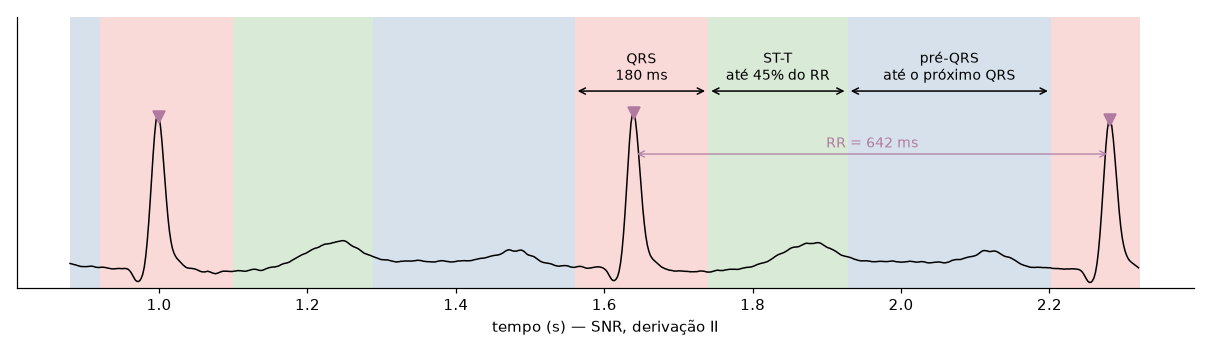
\includegraphics[width=0.62\textwidth]{figs/batimento.png}
\caption{Regiões de cada batimento na derivação II: QRS (vermelho), ST-T (verde) e pré-QRS (azul).}
\label{fig:regioes}
\end{figure}

\section{Faithfulness Estimate}
\textbf{Pergunta.} Retirando \textbf{uma região de cada vez}, a queda na saída do modelo acompanha a importância que o SHAP deu à região? (Alvarez-Melis e Jaakkola, 2018, §5.3.)

\textbf{Por que foi reimplementada.} A configuração usada trocava grupos de 500 pontos pelo valor mínimo do ECG. Num diagnóstico, retirar grupos de importância \textbf{negativa} derrubava a saída quase tanto quanto retirar os de importância positiva (3,06 contra 3,30): a métrica media o dano ao sinal, e não a retirada de informação.

\textbf{Versão atual.} Cada uma das 36 regiões é trocada por uma baseline, uma de cada vez; o valor do ECG é a correlação de Pearson entre as 36 importâncias e as 36 quedas do \textit{logit}. Ela segue o artigo com duas adaptações justificadas: regiões no lugar de atributos isolados (o próprio artigo recomenda unidades de nível mais alto para entradas grandes) e \textit{logit} no lugar da probabilidade, que satura (84\% das retiradas a mudam menos de 0,01). Com a probabilidade, a conclusão é a mesma.

\textbf{Baseline.} O artigo manda trocar o atributo por um ``valor médio'', sem dizer qual. Por isso foram calculadas duas versões: com \textbf{zero} e com a \textbf{média do treino} (média de cada ponto, derivação $\times$ instante, sobre os ECGs de treino). Os resultados coincidem até a terceira casa decimal (global 0,615 nas duas; diferença máxima por classe de 0,001), então os números abaixo valem para as duas. Uma explicação provável é que as duas baselines são quase o mesmo sinal: cada derivação está em z-score, com média zero, e na média do treino os batimentos, que caem em instantes diferentes em cada ECG, tendem a se cancelar.

\textbf{Resultado.} Global de \textbf{0,62}, positiva em todas as classes. Retirar uma região de importância positiva baixa o \textit{logit} em 0,32, em média, e retirar uma de importância negativa o aumenta em 0,34, como se espera de uma explicação fiel.

\section{Max-Sensitivity e Avg-Sensitivity}
\textbf{Pergunta.} Se o ECG mudar um pouquinho, a explicação muda muito? A Max-Sensitivity (Yeh et al., 2019) é a maior mudança da explicação entre várias versões levemente perturbadas do ECG; a Avg-Sensitivity (Bhatt et al., 2020), a média. \textbf{Menor é melhor.}

\textbf{Por que foi reimplementada.} A configuração do Quantus comparava o mapa salvo (50 amostras do GradientSHAP) com mapas refeitos com 20 amostras e outra semente aleatória, somava ruído também ao preenchimento e não descartava perturbações que mudam a predição. Um diagnóstico com 18 ECGs mostrou que o valor obtido era praticamente o mesmo que se obtém \textbf{sem perturbação nenhuma}: a métrica media a aleatoriedade do GradientSHAP, e não a robustez da explicação.

\textbf{Versão atual.} Para cada mapa, 10 perturbações com ruído uniforme de $\pm$0,1 (em escala z-score) somado só ao trecho real do ECG, o raio usado por Yeh et al. Cada ECG perturbado é explicado com a \textbf{mesma configuração e a mesma semente} da explicação original, de modo que a diferença entre os mapas reflete só a perturbação. Perturbações que mudam a predição são descartadas (só 1 de 6\,220 mudou). A distância é a de Yeh et al. (entre mapas normalizados; vai de 0 a 2), calculada nas 36 regiões. Reporta-se também o \textbf{piso}: a distância entre duas execuções do GradientSHAP no mesmo ECG, sem perturbação, com sementes diferentes.

\begin{table}[H]
\centering
\small
\caption{Diagnóstico e resultado global (distância por regiões; “top-2 igual”: os dois mapas têm o mesmo par de regiões principais, que é a explicação usada pela Consistency).}
\begin{tabular}{lrr}
\toprule
\textbf{Comparação} & \textbf{Distância} & \textbf{Top-2 igual} \\
\midrule
Mesmo ECG, outra execução do GradientSHAP (piso) & 0,36 & 67\% \\
ECG perturbado ($\pm$0,1), mesma semente: Max-Sensitivity & 0,07 & 97\% \\
Configuração antiga do Quantus & 0,43 & 56\% \\
\bottomrule
\end{tabular}
\end{table}
\textbf{Resultado.} As explicações são \textbf{robustas}: uma perturbação pequena muda o mapa em 0,07 (numa escala até 2) e mantém o par de regiões principais em 97\% dos casos. Mas o \textbf{piso é cerca de 5 vezes maior}, e isso vale em todos os 622 mapas: duas execuções do GradientSHAP no mesmo ECG concordam no par de regiões principais em só 67\% dos casos. A Max e a Avg ordenam as classes do mesmo jeito, então basta acompanhar uma delas.

\section{Resultados por classe}
\begin{table}[H]
\centering
\small
\caption{F1 e as métricas por classe. Entre parênteses, a posição da classe (1º = melhor; na sensibilidade e no piso, melhor = menor valor). Faithfulness Correlation com grupos de 9 regiões; sensibilidade e piso por regiões.}
\label{tab:res}
\setlength{\tabcolsep}{4pt}
\begin{tabular}{lr rr rr rr rr rr r}
\toprule
\textbf{Classe} & \textbf{Mapas} & \multicolumn{2}{c}{\textbf{F1}} & \multicolumn{2}{c}{\textbf{Consistency}} & \multicolumn{2}{c}{\textbf{Faith.\ Corr.}} & \multicolumn{2}{c}{\textbf{Faith.\ Est.}} & \multicolumn{2}{c}{\textbf{Max-Sens.}} & \textbf{Piso} \\
\midrule
BRD  & 172 & 0,927 & (2º) & 0,64 & (1º) & 0,74 & (1º) & 0,78 & (1º) & 0,058 & (2º) & 0,32 \\
BRE  &  20 & 0,870 & (4º) & 0,25 & (6º) & 0,65 & (2º) & 0,72 & (2º) & 0,047 & (1º) & 0,23 \\
IAVB &  61 & 0,884 & (3º) & 0,45 & (3º) & 0,64 & (3º) & 0,57 & (5º) & 0,064 & (3º) & 0,36 \\
CVP  &  59 & 0,837 & (5º) & 0,26 & (5º) & 0,61 & (4º) & 0,66 & (3º) & 0,073 & (5º) & 0,32 \\
STE  &  14 & 0,596 & (9º) & 0,03 & (9º) & 0,60 & (5º) & 0,57 & (4º) & 0,071 & (4º) & 0,35 \\
AF   & 108 & 0,931 & (1º) & 0,42 & (4º) & 0,54 & (6º) & 0,51 & (7º) & 0,081 & (7º) & 0,35 \\
STD  &  65 & 0,778 & (7º) & 0,51 & (2º) & 0,52 & (7º) & 0,51 & (9º) & 0,085 & (8º) & 0,40 \\
SNR  &  78 & 0,796 & (6º) & 0,21 & (7º) & 0,46 & (9º) & 0,51 & (8º) & 0,077 & (6º) & 0,41 \\
CAP  &  45 & 0,750 & (8º) & 0,14 & (8º) & 0,52 & (8º) & 0,55 & (6º) & 0,096 & (9º) & 0,46 \\
\midrule
\textbf{Global} & 622 & \textbf{0,819} & & \textbf{0,42} & & \textbf{0,61} & & \textbf{0,62} & & \textbf{0,072} & & 0,36 \\
\bottomrule
\end{tabular}
\end{table}
Valores esperados ao acaso na Consistency: global 0,13 (por classe, de 0,02 a 0,23).

\begin{figure}[H]
\centering
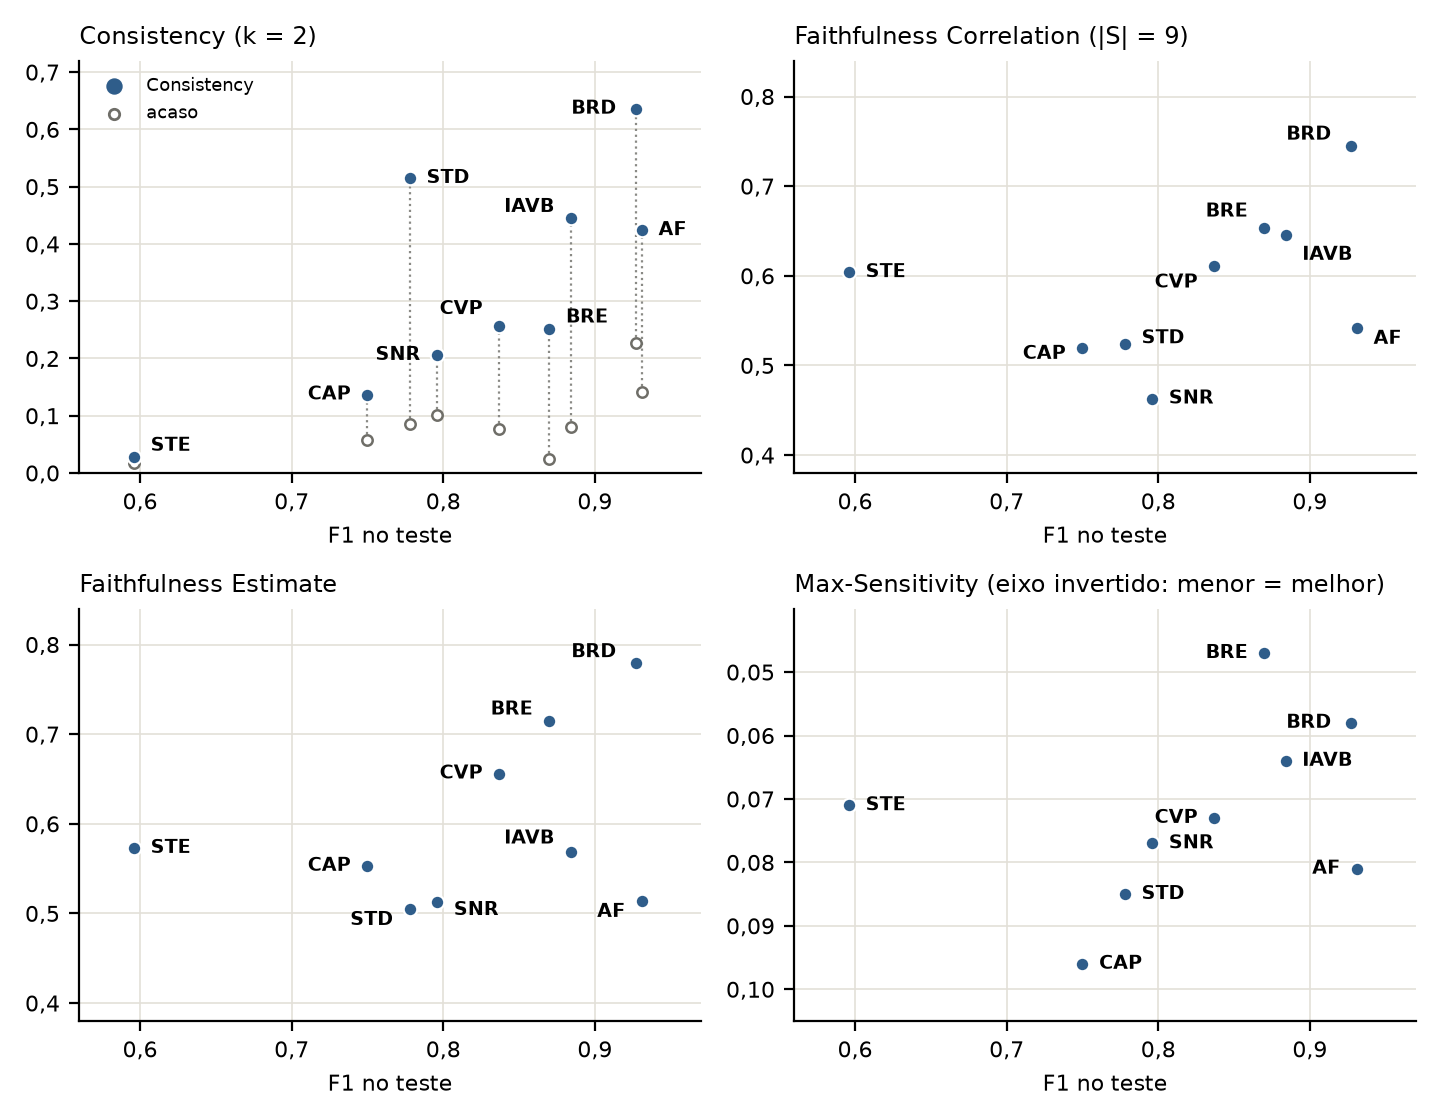
\includegraphics[width=0.92\textwidth]{figs/f1_vs_metricas.png}
\caption{F1 por classe contra cada métrica. Na Max-Sensitivity, o eixo é invertido para que “melhor” fique para cima, como nos outros painéis.}
\label{fig:disp}
\end{figure}

\section{Análise conjunta}
As comparações com o F1 são \textbf{descritivas} (ordenação das classes), sem coeficientes de correlação: as nove classes não são observações independentes nem uma amostra de uma população de classes.

\subsection{O que cada métrica pergunta}
\begin{table}[H]
\centering
\small
\begin{tabularx}{\textwidth}{lXX}
\toprule
\textbf{Dimensão} & \textbf{Pergunta} & \textbf{O que se compara} \\
\midrule
Fidelidade (Faith.\ Corr.\ e Estimate) & A explicação descreve o que o modelo faz? & A explicação com a \textbf{saída do modelo} ao retirar regiões \\
Consistência (Consistency) & ECGs diferentes da mesma classe recebem a mesma explicação? & Explicações de \textbf{ECGs diferentes} \\
Robustez (Max/Avg-Sensitivity) & A explicação se mantém se o ECG mudar um pouquinho? & Explicações de \textbf{versões quase idênticas do mesmo ECG} \\
\bottomrule
\end{tabularx}
\end{table}

\subsection{Dois blocos: fidelidade e robustez de um lado, consistência de outro}
Em princípio são três dimensões. Nos resultados, a robustez acompanha a fidelidade:
\begin{itemize}
    \item As \textbf{4 classes menos robustas} (SNR, AF, STD e CAP) são exatamente as \textbf{4 menos fiéis} na Faithfulness Estimate, e BRE e BRD são as 2 primeiras nas duas. Mapa a mapa, a relação vai na mesma direção (diagnóstico: correlação de postos de $-$0,44 entre sensibilidade e Faithfulness Estimate).
    \item As duas Faithfulness concordam entre si (0,61 e 0,62 no global, ordens parecidas), como já se esperava.
    \item A \textbf{Consistency} segue outra ordem: STD é 2ª na Consistency e fica entre a 7ª e a 9ª posição na fidelidade e na robustez; BRE é 6ª na Consistency e 1ª–2ª nas outras.
\end{itemize}
Leitura: onde o SHAP descreve bem o modelo, ele também é estável; onde descreve pior, também é mais frágil. Já repetir a mesma razão entre ECGs é uma propriedade diferente.

\subsection{Perfis das classes}
\begin{table}[H]
\centering
\small
\begin{tabularx}{\textwidth}{llX}
\toprule
\textbf{Perfil} & \textbf{Classes} & \textbf{Leitura} \\
\midrule
Bom nos dois blocos & BRD, IAVB & Explicações fiéis, robustas e que se repetem entre ECGs. BRD é o caso ideal: QRS de V1 em 87\% dos mapas, o critério clínico do bloqueio de ramo direito. \\
\addlinespace
Fiel e robusto, pouco consistente & BRE, CVP, STE & Cada explicação descreve bem o modelo e é estável, mas a razão varia entre ECGs. \\
\addlinespace
Consistente, menos fiel e robusto & STD, AF & A mesma razão se repete, mas a importância de cada região acompanha pior o modelo e é mais frágil. \\
\addlinespace
Fraco nos dois blocos & SNR, CAP & Explicações menos fiéis, menos robustas e pouco repetidas. \\
\bottomrule
\end{tabularx}
\end{table}

\subsection{A Consistency mistura duas causas}
O GradientSHAP não calcula o mapa de forma exata: ele o estima com 50 sorteios (baselines e ruído), e outro conjunto de sorteios daria um mapa um pouco diferente. O piso mede esse erro de estimativa: em duas execuções no mesmo ECG, o par de regiões principais coincide em só 67\% dos casos.

A Consistency \textbf{capta corretamente} essa variação: as explicações efetivamente geradas são menos consistentes por causa dela, e o valor medido é válido. O que muda é a leitura, porque uma Consistency baixa pode ter duas causas, que a métrica sozinha não separa:
\begin{center}\small
\begin{tabularx}{\linewidth}{lXX}
\toprule
& \textbf{Origem} & \textbf{Relação com a pergunta do TCC} \\
\midrule
A & O modelo usa evidências diferentes em ECGs diferentes da mesma classe & Característica do modelo na classe; faz sentido comparar com o F1 \\ \addlinespace
B & Erro de estimativa do GradientSHAP (50 amostras por mapa) & Característica da configuração do estimador; diminui com mais amostras e não depende de quão bem o modelo classifica a classe \\
\bottomrule
\end{tabularx}
\end{center}
O mesmo erro afeta também a Faithfulness Correlation e a Estimate (importâncias com ruído reduzem a correlação), mas a Consistency tende a ser mais sensível, porque usa um rótulo discreto (o par top-2): um erro pequeno pode trocar o rótulo inteiro.

Como o piso varia entre as classes, ele dá uma indicação de qual causa pesa mais em cada uma:
\begin{itemize}
    \item \textbf{CAP} tem o maior piso (0,46) e Consistency baixa (8ª): parte da inconsistência pode vir da causa B.
    \item \textbf{BRE} tem o menor piso (0,23) e Consistency baixa (6ª): a causa B é pequena, então a inconsistência deve vir principalmente da causa A; as explicações de BRE variam de fato entre ECGs (por exemplo, alternando entre o QRS de V1 e o de V2).
    \item \textbf{STD} tem piso alto (0,40) e mesmo assim Consistency alta (2ª): o padrão de STD se repete apesar da causa B.
\end{itemize}
Assim, a Consistency é mantida como resultado, com o piso ao lado como contexto. Para separar as duas causas, seria preciso gerar os mapas com mais amostras e recalcular a métrica: se a Consistency de uma classe subir, pesava a causa B; se ficar igual, a causa A. Isso tem custo maior de GPU e muda os mapas usados por todas as métricas.

\subsection{O que isso diz sobre a pergunta do TCC}
A qualidade das explicações acompanha o F1 \textbf{em parte}:
\begin{enumerate}
    \item \textbf{Nas pontas há coincidência.} BRD está entre as melhores no F1 e é a melhor ou a segunda em todas as métricas; CAP está entre as piores em tudo.
    \item \textbf{A Consistency é a que mais acompanha o F1.} Fora STD e AF, as posições na Consistency ficam próximas das do F1. Quando o modelo classifica bem uma classe, ele tende a usar uma razão estável entre ECGs.
    \item \textbf{Fidelidade e robustez dependem mais do tipo de classe.} BRE e BRD, definidas pela forma do QRS, têm explicações fiéis e robustas; AF, SNR e CAP, ligadas ao ritmo ou ao batimento como um todo, têm explicações menos fiéis e menos robustas, mesmo com F1 alto no caso de AF. Como as regiões juntam todos os batimentos e não representam o intervalo entre eles, parte disso pode ser uma limitação da própria unidade de medida para classes de ritmo.
    \item \textbf{O pior F1 não tem explicação comum.} STE tem Consistency próxima do acaso, mas fidelidade e robustez intermediárias: cada explicação descreve o modelo, mas o modelo não usa uma razão estável para essa classe (com a ressalva de que são só 14 mapas).
\end{enumerate}

\textbf{Limitações:} um único modelo e uma divisão dos dados; só predições corretas; classes pequenas (STE, BRE) menos estáveis; regiões que favorecem classes de forma local; o ruído do GradientSHAP afeta todos os mapas; as métricas avaliam se o SHAP descreve o modelo, e não se o modelo usa o critério clínico correto.

\section{Situação das métricas}
\begin{table}[H]
\centering
\small
\begin{tabularx}{\textwidth}{lXl}
\toprule
\textbf{Métrica} & \textbf{Artigo de referência} & \textbf{Situação} \\
\midrule
\multicolumn{3}{l}{\textit{Fidelidade}} \\
Consistency & Dasgupta, Frost e Moshkovitz (2022) & Reimplementada e calculada \\
Faithfulness Correlation & Bhatt, Weller e Moura (2020) & Reimplementada e calculada \\
Faithfulness Estimate & Alvarez-Melis e Jaakkola (2018) & \textbf{Reimplementada e calculada (nova)} \\
Sufficiency & Dasgupta, Frost e Moshkovitz (2022) & Retirada \\
Sensitivity-N & Ancona et al. (2018) & Próxima a revisar \\
Selectivity & Montavon, Samek e Müller (2018) & A revisar \\
Infidelity & Yeh et al. (2019) & A revisar \\
\midrule
\multicolumn{3}{l}{\textit{Robustez}} \\
Max- e Avg-Sensitivity & Yeh et al. (2019); Bhatt et al. (2020) & \textbf{Reimplementadas e calculadas (novas)} \\
Local Lipschitz Estimate & Alvarez-Melis e Jaakkola (2018) & A revisar \\
Continuity & Montavon, Samek e Müller (2018) & A revisar \\
RIS e ROS & Agarwal et al. (2022) & A revisar \\
\midrule
\multicolumn{3}{l}{\textit{Complexidade}} \\
Complexity & Bhatt, Weller e Moura (2020) & Analisada; inclusão a decidir \\
\bottomrule
\end{tabularx}
\end{table}

\section{Próximos passos}
\begin{itemize}
    \item Revisar a Sensitivity-N e, depois, as demais métricas de fidelidade e de robustez.
    \item Decidir se os mapas devem ser regerados com mais amostras do GradientSHAP, para reduzir o ruído do estimador.
    \item Decidir a inclusão da complexidade por regiões.
    \item Acrescentar cada nova métrica à análise conjunta, verificando se os dois blocos e os perfis das classes se mantêm.
\end{itemize}

\end{document}
